
%(BEGIN_QUESTION)
% Copyright 2010, Tony R. Kuphaldt, released under the Creative Commons Attribution License (v 1.0)
% This means you may do almost anything with this work of mine, so long as you give me proper credit

Suppose we have an Allen-Bradley model ``SLC 500'' PLC connected to a pair of momentary-contact pushbutton switches and light bulbs as shown in this illustration:

$$\includegraphics[width=15.5cm]{i04628x01.eps}$$

Examine the following relay ladder logic (RLL) program for this Allen-Bradley PLC, determining the statuses of the two lamps provided neither switch A nor switch B is pressed by a human operator:

$$\includegraphics[width=15.5cm]{i04628x02.eps}$$

Finally, draw color highlighting showing how these ``contact'' instructions will appear in an online editor program given the stated input conditions.

\vskip 20pt \vbox{\hrule \hbox{\strut \vrule{} {\bf Suggestions for Socratic discussion} \vrule} \hrule}

\begin{itemize}
\item{} Identify the significance of the labels ``I'' and ``O'' for this PLC's bits.
\item{} Identify the significance of the first and second numbers in each bit label (e.g. the numbers ``1'' and ``2'' in the bit address {\tt I:1/2}, for example).  What pattern do you see as you compare the I/O connections with the respective contact instructions in the PLC program?
\end{itemize}


\underbar{file i04628}
%(END_QUESTION)





%(BEGIN_ANSWER)

Neither output will activate to energize either lamp.

%(END_ANSWER)





%(BEGIN_NOTES)

$$\includegraphics[width=15.5cm]{i04628x03.eps}$$

%INDEX% PLC, relating I/O status to virtual elements

%(END_NOTES)


